\documentclass[10pt,tikz]{standalone}
\usepackage[utf8]{inputenc}
\usepackage{helvet}
\usepackage{amsmath}
\renewcommand{\familydefault}{\sfdefault}
\usepackage{tikz}
\usetikzlibrary{arrows.meta, positioning, calc, shapes.geometric, backgrounds, fit}

\definecolor{emeraldpine}{HTML}{1A4D3E}
\definecolor{harvardcrimson}{HTML}{A51C30}
\definecolor{ethdarkblue}{HTML}{1F407A}
\definecolor{ethpetrol}{HTML}{007A87}
\definecolor{ethbronze}{HTML}{B87333}
\definecolor{ethpurple}{HTML}{5B4B8A}
\definecolor{ink}{HTML}{1A202C}
\definecolor{softink}{HTML}{4A5568}
\definecolor{paleink}{HTML}{A0AEC0}
\definecolor{cardbg}{HTML}{F8FAFC}
\definecolor{shadecolor}{HTML}{F4F6F9}

\begin{document}
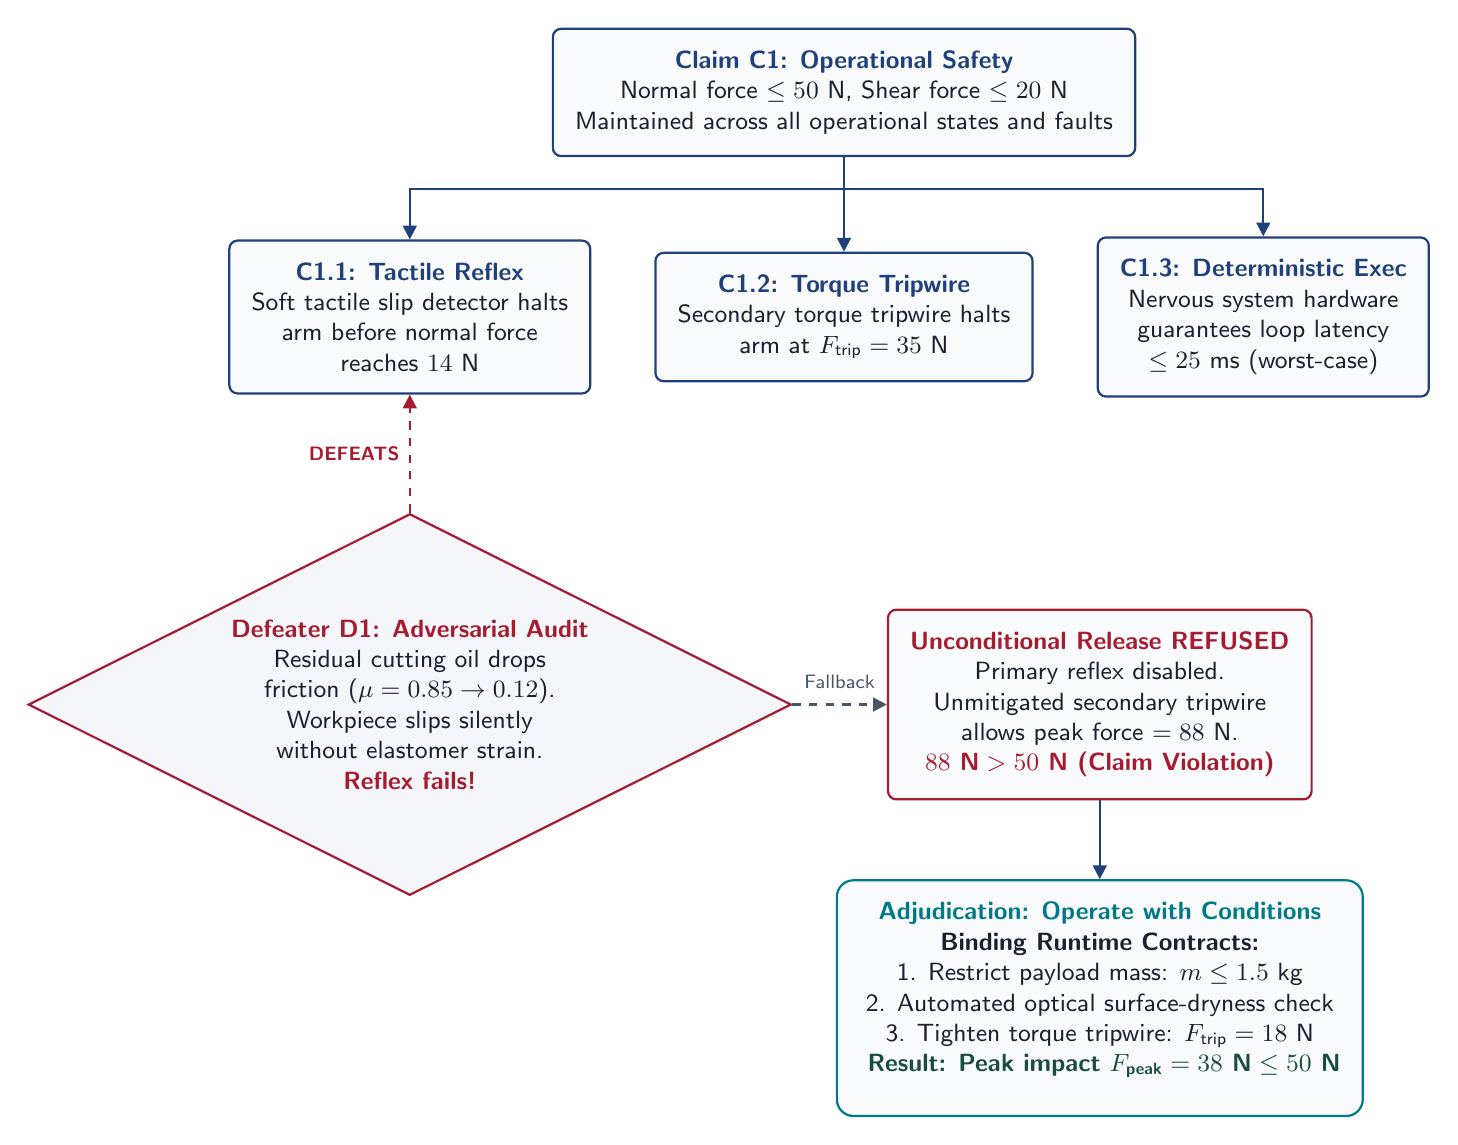
\begin{tikzpicture}[
    >={Triangle[length=5pt, width=5pt]},
    node distance=1.5cm and 0.8cm,
    font=\sffamily\small,
    claim/.style={
        rectangle,
        draw=ethdarkblue,
        fill=cardbg,
        thick,
        rounded corners=3pt,
        inner sep=8pt,
        align=center,
        text=ink
    },
    defeater/.style={
        diamond,
        aspect=2.0,
        draw=harvardcrimson,
        fill=shadecolor,
        thick,
        inner sep=4pt,
        align=center,
        text=ink
    },
    solution/.style={
        rectangle,
        rounded corners=6pt,
        draw=ethpetrol,
        fill=cardbg,
        thick,
        inner sep=8pt,
        align=center,
        text=ink
    },
    refused/.style={
        rectangle,
        draw=harvardcrimson,
        fill=cardbg,
        thick,
        rounded corners=3pt,
        inner sep=8pt,
        align=center,
        text=ink
    },
    link/.style={
        ->,
        thick,
        draw=ethdarkblue
    },
    defeats/.style={
        ->,
        thick,
        draw=harvardcrimson,
        dashed
    }
]

% Level 1
\node[claim] (C1_2) {
    \textbf{\textcolor{ethdarkblue}{C1.2: Torque Tripwire}}\\
    Secondary torque tripwire halts\\
    arm at $F_{\text{trip}} = 35\text{ N}$
};

\node[claim, left=0.8cm of C1_2] (C1_1) {
    \textbf{\textcolor{ethdarkblue}{C1.1: Tactile Reflex}}\\
    Soft tactile slip detector halts\\
    arm before normal force\\
    reaches $14\text{ N}$
};

\node[claim, right=0.8cm of C1_2] (C1_3) {
    \textbf{\textcolor{ethdarkblue}{C1.3: Deterministic Exec}}\\
    Nervous system hardware\\
    guarantees loop latency\\
    $\le 25\text{ ms}$ (worst-case)
};

\node[claim, above=1.2cm of C1_2] (C1) {
    \textbf{\textcolor{ethdarkblue}{Claim C1: Operational Safety}}\\
    Normal force $\le 50\text{ N}$, Shear force $\le 20\text{ N}$\\
    Maintained across all operational states and faults
};

% Connections L1 to L2
\draw[link] (C1.south) -- ++(0,-0.4) -| (C1_1.north);
\draw[link] (C1.south) -- (C1_2.north);
\draw[link] (C1.south) -- ++(0,-0.4) -| (C1_3.north);

% Level 3: Defeater and Refused
\node[defeater, below=1.5cm of C1_1] (D1) {
    \textbf{\textcolor{harvardcrimson}{Defeater D1: Adversarial Audit}}\\
    Residual cutting oil drops\\
    friction ($\mu = 0.85 \rightarrow 0.12$).\\
    Workpiece slips silently\\
    without elastomer strain.\\
    \textbf{\textcolor{harvardcrimson}{Reflex fails!}}
};

\node[refused, right=1.2cm of D1] (Refused) {
    \textbf{\textcolor{harvardcrimson}{Unconditional Release REFUSED}}\\
    Primary reflex disabled.\\
    Unmitigated secondary tripwire\\
    allows peak force $= 88\text{ N}$.\\
    \textbf{\textcolor{harvardcrimson}{$88\text{ N} > 50\text{ N}$ (Claim Violation)}}
};

% Defeater Arrow
\draw[defeats] (D1.north) -- node[left, font=\scriptsize\bfseries\color{harvardcrimson}] {DEFEATS} (C1_1.south);

% Fallback Arrow
\draw[link, dashed, draw=softink] (D1.east) -- node[above=2pt, font=\scriptsize\color{softink}] {Fallback} (Refused.west);

% Level 4: Adjudication
\node[solution, below=1cm of Refused] (Adjudication) {
    \textbf{\textcolor{ethpetrol}{Adjudication: Operate with Conditions}}\\
    \textbf{Binding Runtime Contracts:}\\
    1. Restrict payload mass: $m \le 1.5\text{ kg}$\\
    2. Automated optical surface-dryness check\\
    3. Tighten torque tripwire: $F_{\text{trip}} = 18\text{ N}$\\
    \vspace{2mm}
    \textbf{\textcolor{emeraldpine}{Result: Peak impact $F_{\text{peak}} = 38\text{ N} \le 50\text{ N}$}}
};

\draw[link] (Refused.south) -- (Adjudication.north);

\end{tikzpicture}
\end{document}
